
\documentclass[tikz,border=1pt]{standalone}

\usepackage{amsmath}
\usepackage{xcolor}
\usepackage{tikz}
\usepackage{helvet}
\renewcommand{\familydefault}{\sfdefault}  % Set sans-serif as default

\usetikzlibrary{arrows.meta}
\usetikzlibrary{calc, fit, matrix, positioning}


\tikzstyle{circ}=[circle, draw, minimum size=1.2cm]
\tikzstyle{square}=[rectangle, draw, minimum size=1.2cm]

\begin{document}



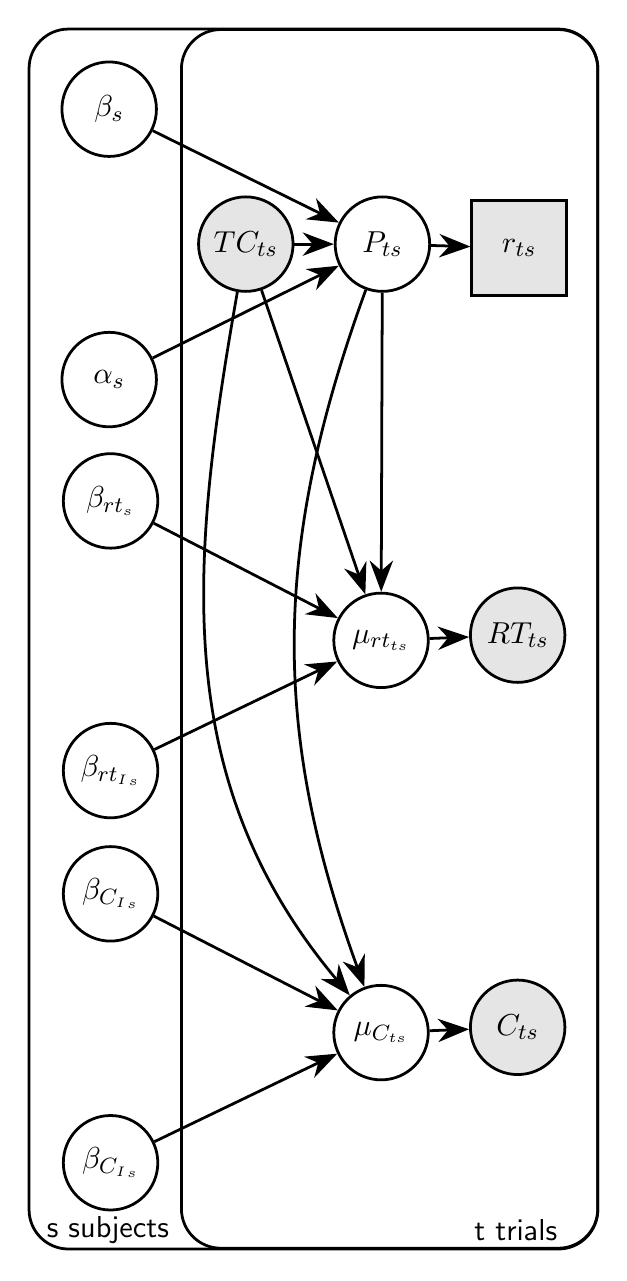
\begin{tikzpicture}
\tikzset{>={Stealth[scale=1.5]}}

\tikzset{every node/.style={font=\sffamily\fontsize{11pt}{12pt}\selectfont}}


%  all lines
\tikzset{every path/.style={line width=1pt}}



% Matrix m0
\matrix (m0) [
    ampersand replacement=\&,
    matrix of math nodes,
    nodes in empty cells,
    column sep=.5cm,
    row sep=0.4cm,
]
{
    |[circ, draw]| \beta_{s} \& | [minimum size=1.2cm, inner sep=0pt, draw=none]| \&| [minimum size=1.2cm, inner sep=0pt, draw=none]| \&| [minimum size=1.2cm, inner sep=0pt, draw=none]|\\
    | [minimum size=1.2cm, inner sep=0pt, draw=none]| \& |[circ, draw, fill=gray!20]| TC_{ts} \&  |[circ, draw]| P_{ts} \& |[square, draw, fill=gray!20]| r_{ts}\\
    |[circ, draw]| \alpha_{s} \& | [minimum size=1.2cm, inner sep=0pt, draw=none]| \&| [minimum size=1.2cm, inner sep=0pt, draw=none]| \&| [minimum size=1.2cm, inner sep=0pt, draw=none]| \\
    % \\
    % |[circ, draw]| \beta_{{C_I}_{s}}\\
    % \\
    % |[circ, draw]| \beta_{{C_I}_{s}} \&\& \& |[circ, draw]| \mu_{{C}_{ts}} \& | [minimum size=1.2cm, inner sep=0pt, draw=none]|\& |[circ, draw, fill=gray!20]| C_{ts}\\
    % \\   
};

% \draw[->, line width=1pt] (m0-1-1) to (m0-2-3);
\draw[->] (m0-1-1) to (m0-2-3);

\draw[->] (m0-3-1) to (m0-2-3);
\draw[->] (m0-2-2) to (m0-2-3);
\draw[->] (m0-2-3) to (m0-2-4);


% Matrix m1 (below m0)
\matrix (m1) [
    ampersand replacement=\&,
    matrix of math nodes,
    nodes in empty cells,
    column sep=.5cm,
    row sep=0.4cm,
    below=0cm of m0
]
{
    |[circ, draw]| \beta_{{rt}_{s}} \&  | [minimum size=1.2cm, inner sep=0pt, draw=none]| \&| [minimum size=1.2cm, inner sep=0pt, draw=none]| \&| [minimum size=1.2cm, inner sep=0pt, draw=none]|\\
    | [minimum size=1.2cm, inner sep=0pt, draw=none]| \&| [minimum size=1.2cm, inner sep=0pt, draw=none]| \& |[circ, draw]| \mu_{{rt}_{ts}} \& |[circ, draw, fill=gray!20]| RT_{ts}\\
    |[circ, draw]| \beta_{{rt_I}_{s}} \& | [minimum size=1.2cm, inner sep=0pt, draw=none]| \&| [minimum size=1.2cm, inner sep=0pt, draw=none]| \&| [minimum size=1.2cm, inner sep=0pt, draw=none]|\\
};

\draw[->] (m1-1-1) to (m1-2-3);
\draw[->] (m1-3-1) to (m1-2-3);
\draw[->] (m1-2-3) to (m1-2-4);
% \draw[->] (m0-2-3) to[out=-120, in=110] (m1-2-3);
\draw[->] (m0-2-3) to (m1-2-3);
\draw[->] (m0-2-2) to (m1-2-3);

% Matrix m2 (below m1)
\matrix (m2) [
    ampersand replacement=\&,
    matrix of math nodes,
    nodes in empty cells,
    column sep=.5cm,
    row sep=0.4cm,
    below=0cm of m1
]
{
    |[circ, draw]| \beta_{{C_I}_{s}}\&  | [minimum size=1.2cm, inner sep=0pt, draw=none]| \&| [minimum size=1.2cm, inner sep=0pt, draw=none]| \&| [minimum size=1.2cm, inner sep=0pt, draw=none]|\\
    | [minimum size=1.2cm, inner sep=0pt, draw=none]| \&| [minimum size=1.2cm, inner sep=0pt, draw=none]| \& |[circ, draw]| \mu_{{C}_{ts}}\& |[circ, draw, fill=gray!20]| C_{ts}\\
    |[circ, draw]| \beta_{{C_I}_{s}}\& | [minimum size=1.2cm, inner sep=0pt, draw=none]| \&| [minimum size=1.2cm, inner sep=0pt, draw=none]| \&| [minimum size=1.2cm, inner sep=0pt, draw=none]|\\
};

\draw[->] (m2-1-1) to (m2-2-3);
\draw[->] (m2-3-1) to (m2-2-3);
\draw[->] (m2-2-3) to (m2-2-4);
\draw[->] (m0-2-3) to[out=-110, in=110] (m2-2-3);
\draw[->] (m0-2-2) to[out=-100, in=130] (m2-2-3);


% Plates
\pgfsetcornersarced{\pgfpoint{5mm}{5mm}}
\node[draw=black, fit=(m0-1-1) (m2-3-4), inner sep=4mm] {};

\pgfsetcornersarced{\pgfpoint{5mm}{5mm}}
\node[draw=black, fit=(m0-1-2) (m2-3-4), inner ysep=4.4mm, inner xsep=3mm, yshift = 0.5mm, xshift = 1mm] {};

\node[rotate=0, anchor=west] at (-3.53,-12.5) {s subjects};
\node[rotate=0, anchor=west] at (1.9,-12.5) {t trials};

\end{tikzpicture}


\end{document}
